\documentclass[12pt,a4paper]{article}

% ─── Page Layout ───────────────────────────────────────────────────────────────
\usepackage[a4paper, margin=0.8in, headheight=14pt]{geometry}

% ─── Fonts (XeLaTeX) ───────────────────────────────────────────────────────────
\usepackage{fontspec}
\usepackage{unicode-math}
\setmainfont{TeX Gyre Pagella}
\setmonofont[Scale=0.88]{TeX Gyre Cursor}
\setmathfont{Latin Modern Math}

% ─── Packages ──────────────────────────────────────────────────────────────────
\usepackage{xcolor}
\usepackage{colortbl}
\usepackage{titlesec}
\usepackage{enumitem}
\usepackage{tabularx}
\usepackage{booktabs}
\usepackage{array}
\usepackage{amsmath}
\usepackage{tikz}
\usetikzlibrary{shapes.geometric, arrows.meta, positioning, calc, fit, decorations.pathreplacing}
\usepackage{tcolorbox}
\tcbuselibrary{skins, breakable}
\usepackage{hyperref}
\usepackage{fancyhdr}
\usepackage{graphicx}
\usepackage{microtype}
\hyphenpenalty=10000
\exhyphenpenalty=10000
\sloppy
\usepackage{caption}
\usepackage{setspace}
\usepackage{multirow}
\usepackage{tocloft}

% ─── Q&A helper ────────────────────────────────────────────────────────────────
\newcommand{\Q}[1]{\textbf{#1}\par\noindent\ignorespaces}

% ─── Colour Palette ────────────────────────────────────────────────────────────
\definecolor{myred}{RGB}{196,30,58}
\definecolor{mydark}{RGB}{30,30,50}
\definecolor{mygreen}{RGB}{14,120,80}
\definecolor{myteal}{RGB}{0,130,140}
\definecolor{myamber}{RGB}{180,100,0}
\definecolor{mypurple}{RGB}{100,30,160}
\definecolor{mygray}{RGB}{246,247,249}
\definecolor{mgframe}{RGB}{180,185,200}
\definecolor{watermark}{RGB}{145,150,170}
\definecolor{hdrred}{RGB}{250,232,235}
\definecolor{hdrgreen}{RGB}{220,244,233}
\definecolor{hdrteal}{RGB}{220,242,244}
\definecolor{hdramber}{RGB}{253,242,215}
\definecolor{hdrpurple}{RGB}{238,228,255}
\definecolor{hdrgray}{RGB}{238,240,245}
\definecolor{rowalt}{RGB}{250,251,253}

% ─── Section Formatting ────────────────────────────────────────────────────────
\titleformat{\section}
  {\large\bfseries\color{myred}}{\thesection.}{0.5em}{}
  [\vspace{1pt}{\color{myred}\rule{\linewidth}{0.8pt}}]
\titleformat{\subsection}
  {\normalsize\bfseries\color{myteal}}{\thesubsection}{0.5em}{}
\titlespacing*{\section}{0pt}{18pt}{7pt}
\titlespacing*{\subsection}{0pt}{11pt}{4pt}

% ─── Paragraph ─────────────────────────────────────────────────────────────────
\setlength{\parindent}{0pt}
\setlength{\parskip}{4pt}

% ─── TOC Styling ───────────────────────────────────────────────────────────────
\renewcommand{\cfttoctitlefont}{\large\bfseries\color{myred}}
\renewcommand{\cftaftertoctitle}{\par\noindent{\color{myred}\rule{\linewidth}{0.8pt}}}
\setlength{\cftbeforetoctitleskip}{0pt}
\setlength{\cftaftertoctitleskip}{6pt}
\renewcommand{\cftsecfont}{\normalsize\bfseries\color{mydark}}
\renewcommand{\cftsecpagefont}{\normalsize\bfseries\color{mydark}}
\renewcommand{\cftsecleader}{\cftdotfill{\cftdotsep}}
\setlength{\cftbeforesecskip}{7pt}
\renewcommand{\cftsubsecfont}{\small\color{mydark}}
\renewcommand{\cftsubsecpagefont}{\small\color{mydark}}
\setlength{\cftbeforesubsecskip}{3pt}
\setlength{\cftsubsecindent}{1.4em}

% ─── Table helpers ─────────────────────────────────────────────────────────────
\renewcommand{\arraystretch}{1.45}
\setlength{\tabcolsep}{6pt}
\arrayrulecolor{mydark}
\newcolumntype{B}[1]{>{\small\bfseries\raggedright\arraybackslash}m{#1}}
\newcolumntype{Y}{>{\small\raggedright\arraybackslash}X}
\renewcommand{\tabularxcolumn}[1]{m{#1}}

% ─── Header / Footer ───────────────────────────────────────────────────────────
\pagestyle{fancy}
\fancyhf{}
\fancyhead[L]{\small\color{myred}\textbf{PE-EC703B}\;\color{mydark}--- Wireless Sensor Networks}
\fancyhead[R]{\small\color{myteal}\textbf{Module 3 Notes}}
\fancyfoot[C]{\small\color{mydark}\thepage}
\fancyfoot[R]{\small\color{watermark}\textit{\copyright\ Biraj}}
\renewcommand{\headrulewidth}{0.5pt}
\renewcommand{\footrulewidth}{0.3pt}

% ─── Hyperref ──────────────────────────────────────────────────────────────────
\hypersetup{
  colorlinks=true, linkcolor=myteal, urlcolor=myteal,
  pdfauthor={Biraj Sarkar},
  pdftitle={PE-EC703B --- Module 3 Notes}
}

% ─── tcolorbox styles ──────────────────────────────────────────────────────────
\tcbset{
  tikzbox/.style={
    colback=mygray, colframe=mgframe, boxrule=0.6pt, arc=4pt,
    left=8pt, right=8pt, top=6pt, bottom=6pt,
    colbacktitle=mgframe, coltitle=mydark,
    fonttitle=\small\bfseries
  },
  defbox/.style={
    colback=hdrgreen, colframe=mygreen, boxrule=0.8pt, arc=4pt,
    left=9pt, right=9pt, top=6pt, bottom=6pt,
    colbacktitle=mygreen, coltitle=white,
    fonttitle=\small\bfseries
  },
  formulabox/.style={
    colback=hdrteal, colframe=myteal, boxrule=0.8pt, arc=4pt,
    left=9pt, right=9pt, top=7pt, bottom=7pt,
    colbacktitle=myteal, coltitle=white,
    fonttitle=\small\bfseries
  },
  examplebox/.style={
    colback=hdramber, colframe=myamber, boxrule=0.8pt, arc=4pt,
    left=9pt, right=9pt, top=6pt, bottom=6pt,
    colbacktitle=myamber, coltitle=white,
    fonttitle=\small\bfseries
  },
  masonbox/.style={
    colback=hdrpurple, colframe=mypurple, boxrule=0.8pt, arc=4pt,
    left=9pt, right=9pt, top=6pt, bottom=6pt,
    colbacktitle=mypurple, coltitle=white,
    fonttitle=\small\bfseries
  },
  exambox/.style={
    colback=hdrpurple, colframe=mypurple, boxrule=1pt, arc=5pt,
    left=10pt, right=10pt, top=8pt, bottom=8pt,
    colbacktitle=mypurple, coltitle=white,
    fonttitle=\bfseries,
    breakable, title after break={\textbf{Frequently Asked / Viva Questions (contd.)}}}
}
\tcbset{breakable}

% ─── TikZ styles ───────────────────────────────────────────────────────────────
\tikzset{
  block/.style={rectangle, draw=myteal, fill=hdrteal,
    text width=2.4cm, align=center, minimum height=0.95cm,
    font=\small, rounded corners=3pt, line width=0.7pt},
  redblock/.style={rectangle, draw=myred, fill=hdrred,
    text width=2.4cm, align=center, minimum height=0.95cm,
    font=\small, rounded corners=3pt, line width=0.7pt},
  netnode/.style={rectangle, draw=myteal, fill=hdrteal,
    text width=1.5cm, align=center, minimum height=0.8cm,
    font=\small, rounded corners=3pt, line width=0.7pt},
  sumjunc/.style={circle, draw=myamber, fill=hdramber,
    minimum size=0.62cm, font=\small, line width=0.8pt},
  snode/.style={circle, draw=mypurple, fill=hdrpurple,
    minimum size=0.55cm, font=\footnotesize, line width=0.7pt},
  arrow/.style={-Stealth, thick, color=mydark},
  redarrow/.style={-Stealth, thick, color=myred},
  line/.style={thick, color=mydark}
}

% ═══════════════════════════════════════════════════════════════════════════════
\begin{document}
% ═══════════════════════════════════════════════════════════════════════════════

\begin{center}
  {\LARGE\bfseries\color{myred} PE-EC703B --- Wireless Sensor Networks}\\[5pt]
  {\normalsize\color{mydark} Semester VII \quad$\bullet$\quad 3L:0T:0P \quad$\bullet$\quad 3 Credits}\\[3pt]
  {\normalsize\color{myteal}\textbf{Module 3 Exam Notes: MAC Protocols, Routing Protocols, IEEE 802.15.4 \& ZigBee}}\\[3pt]
  {\small\color{mydark} CGEC \;$|$\; B.Tech ECE (2023--27) \;$|$\; \textit{Biraj Sarkar}}
\end{center}
\vspace{2pt}
\noindent{\color{myred}\rule{\linewidth}{1.5pt}}
\vspace{2pt}

\hypersetup{linkcolor=mydark}
\tableofcontents
\hypersetup{linkcolor=myteal}
\newpage

% ===============================================================================
\section{MAC Protocols for WSN}
% ===============================================================================

\begin{tcolorbox}[defbox, title={\textbf{MAC Protocol --- Definition}}]
A \textbf{Medium Access Control (MAC) protocol} governs how sensor nodes share the common wireless channel. In WSN, the MAC layer has an additional critical responsibility: \textbf{energy management} --- scheduling the radio's sleep/wake cycle to minimize idle listening, overhearing, and collision-related retransmissions.
\end{tcolorbox}

\subsection{Major Energy Waste Sources at MAC Layer}
\begin{itemize}[leftmargin=*, itemsep=3pt]
  \item \textbf{Idle listening:} Radio is ON but no packet arrives --- most wasteful (equal to RX energy).
  \item \textbf{Overhearing:} A node receives a packet destined for another node.
  \item \textbf{Collision:} Two nodes transmit simultaneously; packets are corrupt and must be retransmitted.
  \item \textbf{Control packet overhead:} RTS/CTS/ACK consume energy without carrying data.
  \item \textbf{Overmitting:} Transmitting to a node not yet ready to receive.
\end{itemize}

% ===============================================================================
\section{Classification of MAC Protocols}
% ===============================================================================

WSN MAC protocols are broadly classified as:

\par\noindent
{\renewcommand{\arraystretch}{1.5}%
\begin{tabularx}{\linewidth}{|B{3.0cm}|Y|Y|Y|}
\hline
\textbf{Category} & \textbf{Mechanism} & \textbf{Advantages} & \textbf{Disadvantages} \\
\hline
\textbf{Contention-based (CSMA family)} & Nodes contend for channel; random back-off on collision & Simple, no coordination needed, handles variable load & Collisions, idle listening, scalability issues \\
\hline
\textbf{Schedule-based (TDMA family)} & Nodes assigned fixed time slots; radio OFF in other slots & Collision-free, predictable energy, no idle listening & Requires synchronization, poor adaptability \\
\hline
\textbf{Hybrid} & Combines TDMA + CSMA dynamically & Balanced energy and adaptability & Complex design \\
\hline
\end{tabularx}}

% ===============================================================================
\section{S-MAC Protocol (Sensor-MAC)}
% ===============================================================================

\begin{tcolorbox}[defbox, title={\textbf{S-MAC --- Definition}}]
\textbf{S-MAC (Sensor-MAC)} is a contention-based MAC protocol for WSN that introduces \textbf{periodic sleep--wake schedules} for all nodes in a neighborhood. Nodes synchronize their schedules, go to sleep during idle periods, and wake up to exchange data only during active periods, dramatically reducing idle-listen energy.
\end{tcolorbox}

\subsection{S-MAC Working Principle}

\begin{enumerate}[leftmargin=*, itemsep=4pt]
  \item \textbf{Listen--Sleep schedule:} Time is divided into frames. Each frame has a \textbf{LISTEN} period and a \textbf{SLEEP} period. All nodes in a cluster share the same schedule.
  \item \textbf{Schedule exchange (SYNC):} On startup, a node listens for SYNC packets. If it hears a neighbor's schedule, it adopts it. Otherwise it creates its own and broadcasts a SYNC packet.
  \item \textbf{Data exchange:} Data is sent only during the LISTEN period using CSMA with RTS/CTS.
  \item \textbf{In-band signaling:} A NAV (Network Allocation Vector) field in RTS/CTS tells neighboring nodes how long to stay asleep (virtual carrier sensing).
  \item \textbf{Message passing:} For long messages, S-MAC uses message passing where a node stays awake for consecutive frames to receive the entire message --- reduces latency.
\end{enumerate}

\subsection{S-MAC Frame Structure}

\begin{tcolorbox}[tikzbox, title={S-MAC Sleep--Wake Schedule}]
\centering
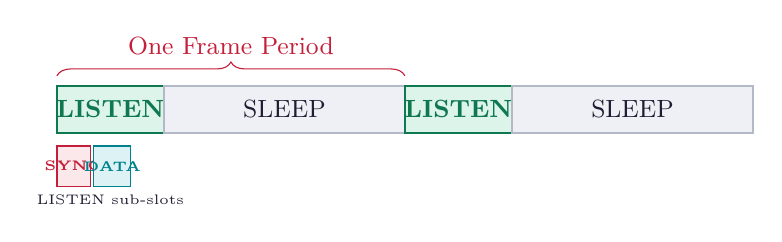
\begin{tikzpicture}[scale=0.85]
  % Frame 1
  \draw[fill=hdrgreen, draw=mygreen, line width=0.7pt] (0,0) rectangle (1.6,0.7);
  \node[font=\small\bfseries, color=mygreen] at (0.8,0.35) {LISTEN};
  \draw[fill=hdrgray, draw=mgframe, line width=0.7pt] (1.6,0) rectangle (5.2,0.7);
  \node[font=\small, color=mydark] at (3.4,0.35) {SLEEP};
  % Frame 2
  \draw[fill=hdrgreen, draw=mygreen, line width=0.7pt] (5.2,0) rectangle (6.8,0.7);
  \node[font=\small\bfseries, color=mygreen] at (6.0,0.35) {LISTEN};
  \draw[fill=hdrgray, draw=mgframe, line width=0.7pt] (6.8,0) rectangle (10.4,0.7);
  \node[font=\small, color=mydark] at (8.6,0.35) {SLEEP};

  % Brace
  \draw[decorate, decoration={brace, amplitude=5pt}, color=myred]
    (0,0.85) -- (5.2,0.85) node[midway, above=4pt, font=\small, color=myred] {One Frame Period};

  % Labels under LISTEN
  \draw[fill=hdrred, draw=myred, line width=0.5pt] (0,-0.8) rectangle (0.5,-0.2);
  \node[font=\tiny\bfseries, color=myred] at (0.25,-0.5) {SYNC};
  \draw[fill=hdrteal, draw=myteal, line width=0.5pt] (0.55,-0.8) rectangle (1.1,-0.2);
  \node[font=\tiny\bfseries, color=myteal] at (0.825,-0.5) {DATA};
  \node[font=\tiny, color=mydark] at (0.8,-1.0) {LISTEN sub-slots};
\end{tikzpicture}
\end{tcolorbox}

\subsection{S-MAC: Advantages and Disadvantages}

\par\noindent
{\renewcommand{\arraystretch}{1.5}%
\begin{tabularx}{\linewidth}{|Y|Y|}
\hline
\textbf{Advantages} & \textbf{Disadvantages} \\
\hline
Reduces idle listening significantly & Fixed duty cycle may waste energy at low traffic \\
\hline
Simple schedule coordination (SYNC packets) & Increased latency due to sleep periods \\
\hline
Collision avoidance via virtual carrier sense (NAV) & Border nodes may follow two schedules, reducing sleep time \\
\hline
Works well in dense, static networks & Not adaptive to varying traffic loads \\
\hline
\end{tabularx}}

% ===============================================================================
\section{B-MAC Protocol (Berkeley-MAC)}
% ===============================================================================

\begin{tcolorbox}[defbox, title={\textbf{B-MAC --- Definition}}]
\textbf{B-MAC (Berkeley-MAC)} is a contention-based MAC protocol that uses \textbf{Low-Power Listening (LPL)} (also called \textbf{preamble sampling}) to reduce idle-listen energy. A node wakes up briefly at intervals to check for channel activity (preamble) and only stays awake if it detects a transmission directed to it.
\end{tcolorbox}

\subsection{B-MAC Low-Power Listening (LPL) Mechanism}

\begin{enumerate}[leftmargin=*, itemsep=4pt]
  \item \textbf{Receiver side:} Each node wakes up periodically (every check interval $T_c$) for a short duration ($\sim$1 ms), samples the channel using Clear Channel Assessment (CCA).
  \begin{itemize}
    \item If channel is idle: back to sleep.
    \item If channel is busy: stay awake and receive the full packet.
  \end{itemize}
  \item \textbf{Sender side:} Before data, the sender transmits a \textbf{long preamble} of duration $\geq T_c$ (the check interval). This ensures the receiver wakes up at least once and detects the preamble.
  \item After detecting the preamble, the receiver stays awake and receives the data packet.
\end{enumerate}

\begin{tcolorbox}[tikzbox, title={B-MAC Low-Power Listening --- Timing}]
\centering
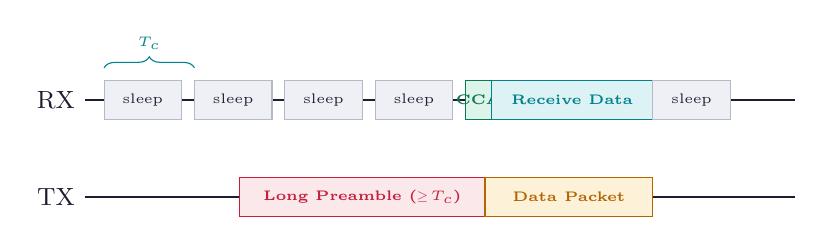
\begin{tikzpicture}[scale=0.82]
  % Receiver timeline
  \draw[thick, color=mydark] (0,1.5) -- (11,1.5);
  \node[left, font=\small, color=mydark] at (0,1.5) {RX};
  % Sleep pulses
  \foreach \x in {0.3, 1.7, 3.1, 4.5} {
    \draw[fill=hdrgray, draw=mgframe] (\x,1.2) rectangle (\x+1.2,1.8);
    \node[font=\tiny, color=mydark] at (\x+0.6,1.5) {sleep};
  }
  % Wake up sample
  \draw[fill=hdrgreen, draw=mygreen] (5.9,1.2) rectangle (6.3,1.8);
  \node[font=\tiny\bfseries, color=mygreen] at (6.1,1.5) {CCA};
  % Stay awake + receive
  \draw[fill=hdrteal, draw=myteal] (6.3,1.2) rectangle (8.8,1.8);
  \node[font=\tiny\bfseries, color=myteal] at (7.55,1.5) {Receive Data};
  % Back to sleep
  \draw[fill=hdrgray, draw=mgframe] (8.8,1.2) rectangle (10.0,1.8);
  \node[font=\tiny, color=mydark] at (9.4,1.5) {sleep};

  % Sender timeline
  \draw[thick, color=mydark] (0,0) -- (11,0);
  \node[left, font=\small, color=mydark] at (0,0) {TX};
  \draw[fill=hdrred, draw=myred] (2.4,-0.3) rectangle (6.2,0.3);
  \node[font=\tiny\bfseries, color=myred] at (4.3,0.0) {Long Preamble ($\geq T_c$)};
  \draw[fill=hdramber, draw=myamber] (6.2,-0.3) rectangle (8.8,0.3);
  \node[font=\tiny\bfseries, color=myamber] at (7.5,0.0) {Data Packet};

  % Brace for check interval
  \draw[decorate, decoration={brace, amplitude=4pt}, color=myteal]
    (0.3,2.0) -- (1.7,2.0) node[midway, above=3pt, font=\tiny, color=myteal] {$T_c$};
\end{tikzpicture}
\end{tcolorbox}

\subsection{B-MAC vs S-MAC}

\par\noindent
{\renewcommand{\arraystretch}{1.5}%
\begin{tabularx}{\linewidth}{|B{3.0cm}|Y|Y|}
\hline
\textbf{Parameter} & \textbf{S-MAC} & \textbf{B-MAC} \\
\hline
\textbf{Approach} & Synchronized sleep schedules & Asynchronous preamble sampling \\
\hline
\textbf{Synchronization} & Required (SYNC packets) & Not required \\
\hline
\textbf{Latency} & Higher (must wait for LISTEN period) & Lower (no schedule dependency) \\
\hline
\textbf{Preamble overhead} & Short & Long (= check interval) \\
\hline
\textbf{Adaptability} & Fixed duty cycle & Check interval tunable per traffic load \\
\hline
\textbf{Complexity} & Moderate & Low \\
\hline
\end{tabularx}}

% ===============================================================================
\section{IEEE 802.15.4 Standard}
% ===============================================================================

\begin{tcolorbox}[defbox, title={\textbf{IEEE 802.15.4 --- Definition}}]
\textbf{IEEE 802.15.4} is the wireless standard defining the \textbf{Physical (PHY)} and \textbf{MAC} layers for Low-Rate Wireless Personal Area Networks (LR-WPANs). It is the foundation protocol used by ZigBee, 6LoWPAN, Thread, and WirelessHART. It targets low data rate, low power, and low cost sensor/actuator applications.
\end{tcolorbox}

\subsection{Key Specifications of IEEE 802.15.4}

\par\noindent
{\renewcommand{\arraystretch}{1.5}%
\begin{tabularx}{\linewidth}{|B{3.4cm}|Y|}
\hline
\textbf{Parameter} & \textbf{Value / Description} \\
\hline
\textbf{Frequency band} & 2.4 GHz (global), 915 MHz (Americas), 868 MHz (Europe) \\
\hline
\textbf{Data rate} & 250 kbps (2.4 GHz); 40 kbps (915 MHz); 20 kbps (868 MHz) \\
\hline
\textbf{Range} & 10--100 m (LOS); 10--30 m indoor \\
\hline
\textbf{TX power} & $-3$ dBm to $+3$ dBm (1--2 mW) \\
\hline
\textbf{Modulation} & O-QPSK (2.4 GHz), BPSK (868/915 MHz) \\
\hline
\textbf{Channels} & 16 channels at 2.4 GHz (Ch. 11--26, 5 MHz spacing) \\
\hline
\textbf{Addressing} & 16-bit short or 64-bit extended IEEE address \\
\hline
\textbf{Network topology} & Star or peer-to-peer (mesh) \\
\hline
\textbf{Security} & AES-128 encryption optional \\
\hline
\end{tabularx}}

\subsection{Device Types in IEEE 802.15.4}
\begin{itemize}[leftmargin=*, itemsep=3pt]
  \item \textbf{Full Function Device (FFD):} Can act as coordinator, router, or end device. Supports all MAC functions.
  \item \textbf{Reduced Function Device (RFD):} Simplified device; can only communicate with a coordinator. Cannot relay packets. Lower cost, lower power.
  \item \textbf{PAN Coordinator:} The master FFD of the network; manages the PAN (Personal Area Network), assigns addresses, and generates beacon frames.
\end{itemize}

\subsection{Superframe Structure}

IEEE 802.15.4 optionally uses a \textbf{beacon-enabled superframe} structure for scheduled access:

\begin{itemize}[leftmargin=*, itemsep=3pt]
  \item \textbf{Beacon:} Sent by PAN coordinator to synchronize all devices.
  \item \textbf{CAP (Contention Access Period):} CSMA-CA based contention slots for general data.
  \item \textbf{CFP (Contention-Free Period):} Guaranteed Time Slots (GTS) assigned to specific devices --- collision-free, low latency.
  \item \textbf{Inactive period:} All nodes sleep; radio off.
\end{itemize}

% ===============================================================================
\section{ZigBee}
% ===============================================================================

\begin{tcolorbox}[defbox, title={\textbf{ZigBee --- Definition}}]
\textbf{ZigBee} is a high-level wireless communication protocol stack built on top of IEEE 802.15.4 (PHY + MAC layers). It adds the \textbf{Network Layer (NWK)} and \textbf{Application Layer (APL)} to enable mesh networking, self-healing, multi-hop routing, and device/service discovery for IoT and WSN applications.
\end{tcolorbox}

\subsection{ZigBee Protocol Stack}

\begin{tcolorbox}[tikzbox, title={ZigBee Protocol Stack Layers}]
\centering
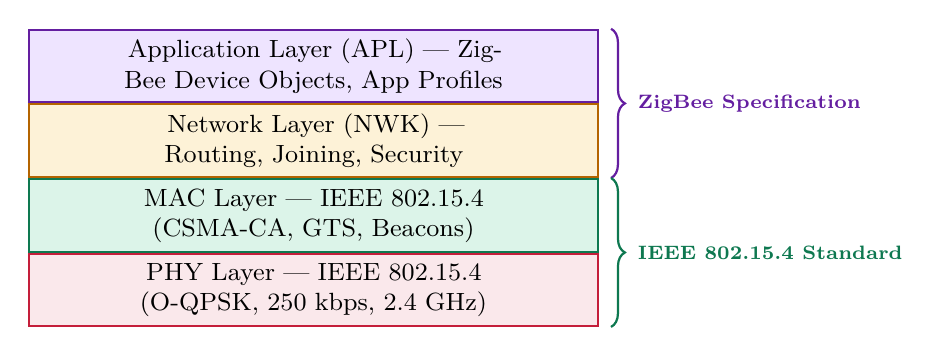
\begin{tikzpicture}[node distance=0cm,
  layer/.style={rectangle, draw=myteal, fill=hdrteal, text width=7cm,
    align=center, minimum height=0.65cm, font=\small, line width=0.7pt}]
  \node[layer, fill=hdrpurple, draw=mypurple] (apl) {Application Layer (APL) --- ZigBee Device Objects, App Profiles};
  \node[layer, fill=hdramber, draw=myamber, below=0cm of apl] (nwk) {Network Layer (NWK) --- Routing, Joining, Security};
  \node[layer, fill=hdrgreen, draw=mygreen, below=0cm of nwk] (mac) {MAC Layer --- IEEE 802.15.4 (CSMA-CA, GTS, Beacons)};
  \node[layer, fill=hdrred, draw=myred, below=0cm of mac] (phy) {PHY Layer --- IEEE 802.15.4 (O-QPSK, 250 kbps, 2.4 GHz)};

  % Grouping braces on the right side
  \draw[decorate, decoration={brace, amplitude=5pt}, thick, color=mypurple]
    ($(apl.north east) + (0.15,0)$) -- ($(nwk.south east) + (0.15,0)$)
    node[midway, right=6pt, font=\scriptsize\bfseries, color=mypurple] {ZigBee Specification};

  \draw[decorate, decoration={brace, amplitude=5pt}, thick, color=mygreen]
    ($(mac.north east) + (0.15,0)$) -- ($(phy.south east) + (0.15,0)$)
    node[midway, right=6pt, font=\scriptsize\bfseries, color=mygreen] {IEEE 802.15.4 Standard};
\end{tikzpicture}
\end{tcolorbox}

\subsection{ZigBee Device Types}
\begin{itemize}[leftmargin=*, itemsep=3pt]
  \item \textbf{ZigBee Coordinator (ZC):} One per network; initiates network formation, stores network map, and bridges to other networks.
  \item \textbf{ZigBee Router (ZR):} Participates in routing; relays data for other nodes; always-on (not battery-optimized).
  \item \textbf{ZigBee End Device (ZED):} Leaf node; communicates only with its parent (coordinator or router); can sleep aggressively; lowest power.
\end{itemize}

\subsection{ZigBee Network Topologies}
\begin{itemize}[leftmargin=*, itemsep=3pt]
  \item \textbf{Star:} All devices communicate directly to the coordinator. Simple, limited range.
  \item \textbf{Tree (Cluster tree):} Hierarchical network; data flows up the tree toward the coordinator. Scalable.
  \item \textbf{Mesh:} Any router can communicate with any other router. Self-healing; most robust; supports AODV-based routing.
\end{itemize}

% ===============================================================================
\section{Routing Protocols for WSN}
% ===============================================================================

Routing in WSN must be energy-aware, since the network lifetime depends on balancing energy consumption across nodes.

\subsection{Flooding and Gossiping}

\begin{itemize}[leftmargin=*, itemsep=3pt]
  \item \textbf{Flooding:} A node broadcasts a packet to all neighbors; each receiving node rebroadcasts to its neighbors, and so on. Simple but causes \textbf{implosion} (same data arrives at a node multiple times), \textbf{overlap} (nearby nodes sense same region and send duplicate data), and \textbf{resource blindness} (does not consider node energy).
  \item \textbf{Gossiping:} Instead of broadcasting, a node randomly selects one neighbor and forwards the packet. Reduces implosion but creates random latency.
\end{itemize}

\subsection{SPIN (Sensor Protocols for Information via Negotiation)}

\begin{tcolorbox}[defbox, title={\textbf{SPIN --- Definition}}]
\textbf{SPIN} is a data-centric routing protocol that uses \textbf{metadata negotiation} to eliminate redundant transmissions. Nodes advertise data descriptors (meta-data) before sending actual data, and only nodes that do not have the data request it.
\end{tcolorbox}

SPIN uses three message types:
\begin{itemize}[leftmargin=*, itemsep=2pt]
  \item \textbf{ADV:} Advertisement --- ``I have new data with this descriptor''.
  \item \textbf{REQ:} Request --- ``I want that data''.
  \item \textbf{DATA:} Actual data payload.
\end{itemize}

\subsection{Directed Diffusion}

\begin{tcolorbox}[defbox, title={\textbf{Directed Diffusion --- Definition}}]
\textbf{Directed Diffusion} is a data-centric, interest-driven routing protocol where the sink \textbf{floods interests} (queries) into the network. Sensor nodes that have matching data respond by sending data along the gradient (path) that was set up by the interest. Reinforcement is used to select the best path.
\end{tcolorbox}

Three phases:
\begin{enumerate}[leftmargin=*, itemsep=3pt]
  \item \textbf{Interest propagation:} Sink broadcasts interest (query) with parameters (attribute=value pairs, duration, frequency).
  \item \textbf{Gradient setup:} Each intermediate node records the direction of the interest source and sets up a gradient toward the sink.
  \item \textbf{Data delivery + Path reinforcement:} Data flows back along gradients. The sink reinforces the best-quality path by increasing data rate on that path; other gradients are suppressed.
\end{enumerate}

\subsection{LEACH Protocol (Low-Energy Adaptive Clustering Hierarchy)}

\begin{tcolorbox}[defbox, title={\textbf{LEACH --- Definition}}]
\textbf{LEACH} is a hierarchical, cluster-based routing protocol for WSN that distributes energy load by rotating the \textbf{Cluster Head (CH)} role among all nodes in rounds. Each CH aggregates data from its cluster members and forwards compressed data to the base station via single-hop.
\end{tcolorbox}

\subsubsection*{LEACH Operation: Two Phases per Round}

\textbf{Phase 1 --- Setup Phase:}
\begin{itemize}[leftmargin=*, itemsep=2pt]
  \item Each node decides to become a CH with probability $p$:
\end{itemize}

\begin{tcolorbox}[formulabox, title={\textbf{LEACH --- Cluster Head Probability}}]
\[
P(n) = \begin{cases}
\dfrac{p}{1 - p \cdot (r \bmod \frac{1}{p})} & \text{if } n \notin G \\
0 & \text{if } n \in G
\end{cases}
\]
where $p$ = desired fraction of CHs (typically 0.05 = 5\%), $r$ = current round number, $G$ = set of nodes that were CHs in the last $1/p$ rounds.

\textbf{Optimal CH fraction:} $p_{\text{opt}} = \sqrt{\dfrac{A}{2\pi}} \cdot \dfrac{1}{d_{BS}} \cdot \sqrt{\dfrac{\varepsilon_{\text{fs}}}{\varepsilon_{\text{mp}}}}$

where $A$ = field area, $d_{BS}$ = distance to base station.
\end{tcolorbox}

\begin{itemize}[leftmargin=*, itemsep=2pt]
  \item Nodes that become CHs broadcast an advertisement. Non-CH nodes join the nearest CH (based on RSSI).
  \item CH creates a TDMA schedule for its cluster members.
\end{itemize}

\textbf{Phase 2 --- Steady-State Phase:}
\begin{itemize}[leftmargin=*, itemsep=2pt]
  \item Cluster members transmit data in their assigned TDMA slot; radio is OFF in other slots.
  \item CH aggregates received data and transmits compressed aggregate to base station using long-range radio.
  \item After a fixed number of frames, a new setup phase begins with new CH selection.
\end{itemize}

\begin{tcolorbox}[tikzbox, title={LEACH Cluster Formation Diagram}]
\centering
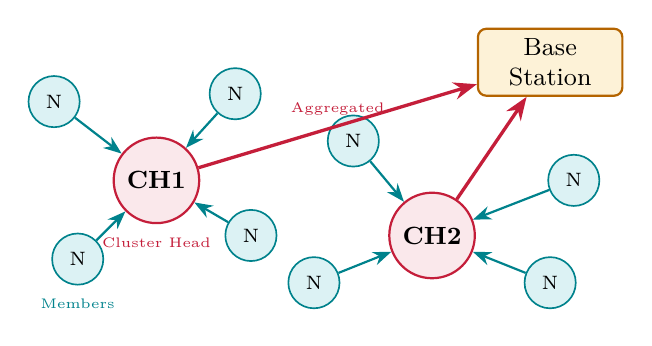
\begin{tikzpicture}[node distance=0.4cm,
  chnode/.style={circle, draw=myred, fill=hdrred, minimum size=1.0cm, font=\small\bfseries, line width=0.8pt},
  mnode/.style={circle, draw=myteal, fill=hdrteal, minimum size=0.65cm, font=\scriptsize, line width=0.6pt},
  bsnode/.style={rectangle, draw=myamber, fill=hdramber, text width=1.6cm, align=center, minimum height=0.85cm, font=\small, rounded corners=3pt, line width=0.8pt}]

  % Base Station
  \node[bsnode] (bs) at (6.5,3.0) {Base Station};

  % Cluster 1 CH
  \node[chnode] (ch1) at (1.5, 1.5) {CH1};
  % Cluster 1 members
  \node[mnode] (m11) at (0.2, 2.5) {N};
  \node[mnode] (m12) at (0.5, 0.5) {N};
  \node[mnode] (m13) at (2.5, 2.6) {N};
  \node[mnode] (m14) at (2.7, 0.8) {N};

  % Cluster 2 CH
  \node[chnode] (ch2) at (5.0, 0.8) {CH2};
  % Cluster 2 members
  \node[mnode] (m21) at (3.5, 0.2) {N};
  \node[mnode] (m22) at (4.0, 2.0) {N};
  \node[mnode] (m23) at (6.5, 0.2) {N};
  \node[mnode] (m24) at (6.8, 1.5) {N};

  % Member to CH arrows
  \draw[arrow, color=myteal] (m11) -- (ch1);
  \draw[arrow, color=myteal] (m12) -- (ch1);
  \draw[arrow, color=myteal] (m13) -- (ch1);
  \draw[arrow, color=myteal] (m14) -- (ch1);
  \draw[arrow, color=myteal] (m21) -- (ch2);
  \draw[arrow, color=myteal] (m22) -- (ch2);
  \draw[arrow, color=myteal] (m23) -- (ch2);
  \draw[arrow, color=myteal] (m24) -- (ch2);

  % CH to BS arrows
  \draw[redarrow, line width=1.2pt] (ch1) -- (bs) node[midway, above, font=\tiny, color=myred] {Aggregated};
  \draw[redarrow, line width=1.2pt] (ch2) -- (bs);

  % Labels
  \node[font=\tiny, color=myred, below=0.05cm of ch1] {Cluster Head};
  \node[font=\tiny, color=myteal, below=0.05cm of m12] {Members};
\end{tikzpicture}
\end{tcolorbox}

\subsection{TEEN and APTEEN Protocols}

For applications with time-critical events, standard proactive clustering like LEACH is inefficient because it transmits data periodically even when there is no change in the sensed environment. Hierarchical routing has reactive and hybrid extensions:

\begin{tcolorbox}[defbox, title={\textbf{TEEN (Threshold sensitive Energy Efficient sensor Network) --- Definition}}]
\textbf{TEEN} is a \textbf{reactive} hierarchical routing protocol designed for time-critical applications. Motes sense their environment continuously, but only transmit data to their cluster heads if the sensed value crosses a \textbf{Hard Threshold ($H_T$)} (to trigger on events of interest) and changes by an amount equal to or greater than a \textbf{Soft Threshold ($S_T$)} (to reduce transmission of small, insignificant fluctuations).
\end{tcolorbox}

\textbf{TEEN Threshold Conditions for Transmission:}
Let $V_{\text{sensed}}$ be the current sensed value, and $V_{\text{last\_tx}}$ be the value of the last transmitted data. A node transmits if and only if:
\[
(V_{\text{sensed}} > H_T) \quad \land \quad (|V_{\text{sensed}} - V_{\text{last\_tx}}| \geq S_T)
\]
\begin{itemize}[leftmargin=*, itemsep=3pt]
  \item \textbf{Hard Threshold ($H_T$):} The absolute value above which a sensor node must turn on its transmitter and report (e.g., Temperature $> 60^\circ$C).
  \item \textbf{Soft Threshold ($S_T$):} A small change in the value of the sensed attribute that triggers the node to transmit again (e.g., change of $\ge 2^\circ$C).
\end{itemize}

\begin{tcolorbox}[defbox, title={\textbf{APTEEN (Adaptive Periodic Threshold sensitive Energy Efficient) --- Definition}}]
\textbf{APTEEN} is a \textbf{hybrid} protocol that extends TEEN to support both periodic (proactive) data collection and event-driven (reactive) transmissions. It allows the user to specify a \textbf{Count Time ($T_C$)}: if a node does not send data for a duration equal to $T_C$, it is forced to transmit its current reading, ensuring the user receives regular heartbeats.
\end{tcolorbox}

\textbf{Comparison: LEACH vs. TEEN vs. APTEEN}

\par\noindent
{\renewcommand{\arraystretch}{1.4}%
\begin{tabularx}{\linewidth}{|B{2.8cm}|Y|Y|Y|}
\hline
\textbf{Parameter} & \textbf{LEACH} & \textbf{TEEN} & \textbf{APTEEN} \\
\hline
\textbf{Network Type} & Proactive (periodic) & Reactive (event-driven) & Hybrid (periodic + event) \\
\hline
\textbf{Data transmission} & Continuous at time slots & Only when thresholds met & Periodic + threshold triggers \\
\hline
\textbf{Energy efficiency} & Moderate & Very High & High \\
\hline
\textbf{Delay} & Higher (scheduled) & Minimal (immediate TX) & Minimal for events \\
\hline
\textbf{Best suited for} & Constant monitoring & Disaster/fire detection & Dynamic query systems \\
\hline
\end{tabularx}}

\subsection{Location-Based (Geographic) Routing Protocols}

Geographic routing protocols use geographic coordinates (localization or GPS) to route data, eliminating the need to maintain routing tables or flood interests.

\begin{tcolorbox}[defbox, title={\textbf{GEAR (Geographical and Energy-Aware Routing) --- Definition}}]
\textbf{GEAR} is a location-based routing protocol that routes queries to a target region using geographic coordinates and remaining energy levels of neighbors. It replaces interest flooding (in Directed Diffusion) with localized geographic forwarding to the target region, saving significant energy.
\end{tcolorbox}

\textbf{GEAR Forwarding Strategy:}
\begin{itemize}[leftmargin=*, itemsep=2pt]
  \item A node forwards packets to the neighbor closest to the target region that has high remaining energy.
  \item If a node encounters a ``hole'' (no neighbor is closer to the target than itself), it routes using a \textbf{learned cost} based on neighbor energy and distance.
\end{itemize}

\begin{tcolorbox}[defbox, title={\textbf{GAF (Geographic Adaptive Fidelity) --- Definition}}]
\textbf{GAF} is an energy-conserving location-based routing protocol that divides the network area into a \textbf{virtual grid}. Since all nodes within a grid cell can route packets to adjacent cells equally, GAF keeps only \textbf{one node active} in each cell while putting all other nodes in a low-power sleep state, maximizing network lifetime.
\end{tcolorbox}

\textbf{GAF Grid Size Constraint:}
To ensure any node in a grid cell $(x, y)$ can communicate with any node in adjacent cells (like $(x+1, y)$), the grid cell size $r$ must satisfy:
\[
r \leq \frac{R}{\sqrt{5}}
\]
where $R$ is the wireless transmission range of the nodes.

% ===============================================================================
\newpage
\begin{center}
  {\large\bfseries\color{myred} Quick Revision --- Module 3}\\[3pt]
  {\small\color{mydark} MAC \& Routing Protocols $|$ PE-EC703B}
\end{center}
\noindent{\color{myred}\rule{\linewidth}{1.2pt}}
\vspace{4pt}

\begin{tcolorbox}[formulabox, title={\textbf{Key Formulas at a Glance}}]
\renewcommand{\arraystretch}{1.4}
\begin{tabularx}{\linewidth}{B{5.0cm} X}
LEACH CH Probability & $P(n) = \displaystyle\frac{p}{1 - p \cdot (r \bmod \frac{1}{p})}$ for non-recent CH nodes; 0 otherwise \\[4pt]
Optimal CH Fraction & $p_{\text{opt}} \propto \displaystyle\frac{1}{d_{BS}} \cdot \sqrt{\frac{\varepsilon_{\text{fs}}}{\varepsilon_{\text{mp}}}}$ \\[4pt]
TEEN Tx Condition & $(V_{\text{sensed}} > H_T) \land (|V_{\text{sensed}} - V_{\text{last\_tx}}| \geq S_T)$ \\[4pt]
GAF Grid Cell Constraint & $r \leq \displaystyle\frac{R}{\sqrt{5}}$ \quad ($R$ = transmission range) \\[4pt]
B-MAC Preamble Length & $T_{\text{preamble}} \geq T_{\text{check}}$ \quad ($T_{\text{check}}$ = receiver check interval)
\end{tabularx}
\end{tcolorbox}

\begin{tcolorbox}[defbox, title={\textbf{One-Line Definitions}}]
\begin{itemize}[leftmargin=*, itemsep=3pt]
  \item \textbf{S-MAC:} Synchronized sleep-wake MAC; nodes share a schedule and sleep during idle periods.
  \item \textbf{B-MAC:} Preamble sampling MAC; receiver wakes briefly to check for long preamble before receiving.
  \item \textbf{IEEE 802.15.4:} PHY+MAC standard for LR-WPAN; 250 kbps at 2.4 GHz; foundation of ZigBee.
  \item \textbf{ZigBee:} Network+application layer stack on IEEE 802.15.4; mesh routing, self-healing, IoT standard.
  \item \textbf{SPIN:} Metadata negotiation protocol --- nodes advertise before sending to avoid redundant transmissions.
  \item \textbf{Directed Diffusion:} Interest-driven data-centric routing; sink floods interests, nodes set up gradients.
  \item \textbf{LEACH:} Cluster-based hierarchical routing; rotates cluster head role to distribute energy consumption.
  \item \textbf{TEEN:} Reactive hierarchical routing; transmits only when sensed parameters cross thresholds.
  \item \textbf{APTEEN:} Hybrid hierarchical routing; combines periodic reporting (Count Time) and threshold-triggered event reporting.
  \item \textbf{GEAR:} Location-based routing routing queries to target region using coordinates and remaining energy.
  \item \textbf{GAF:} Grid-based geographic routing; keeps only one active node per grid cell while others sleep.
\end{itemize}
\end{tcolorbox}

\begin{tcolorbox}[exambox, title={\textbf{Frequently Asked / Viva Questions}}]
\begin{enumerate}[topsep=0pt, label=\textbf{Q\arabic*.}, itemsep=5pt]
  \item \Q{Explain the working of S-MAC protocol.}
  S-MAC introduces synchronized sleep-wake scheduling. Nodes exchange SYNC packets to agree on a schedule with a fixed LISTEN period and a longer SLEEP period per frame. During LISTEN, data is exchanged using CSMA with RTS/CTS and NAV virtual carrier sense. During SLEEP, the radio is OFF saving idle-listen energy.

  \item \Q{What is Low-Power Listening (LPL) in B-MAC?}
  In B-MAC, each receiver wakes up briefly every $T_c$ (check interval) and performs CCA (Clear Channel Assessment). If it detects a long preamble (of duration $\geq T_c$ sent by the transmitter), it stays awake to receive the full data packet. Otherwise it goes back to sleep.

  \item \Q{Compare S-MAC and B-MAC.}
  S-MAC uses \textit{synchronous} fixed sleep schedules (requires SYNC overhead, higher latency). B-MAC uses \textit{asynchronous} preamble sampling (no synchronization needed, lower latency, but long preamble wastes TX energy). B-MAC is more adaptive; S-MAC is better for dense static networks.

  \item \Q{What is IEEE 802.15.4? List its key specifications.}
  IEEE 802.15.4 is the PHY+MAC standard for Low-Rate WPAN. Key specs: 250 kbps at 2.4 GHz (O-QPSK), 16 channels (Ch.11--26), 10--100 m range, $\sim$1--2 mW TX power, AES-128 optional security, 16-bit or 64-bit addressing, star or mesh topology. It is the PHY/MAC base for ZigBee, 6LoWPAN, Thread.

  \item \Q{What is ZigBee and how does it relate to IEEE 802.15.4?}
  ZigBee is a higher-layer protocol stack that adds a Network Layer (mesh routing, AODV, joining) and Application Layer (profiles, device objects) on top of IEEE 802.15.4 PHY and MAC. ZigBee defines three device types: Coordinator (one per network), Router (always-on relay), and End Device (sleepy leaf node).

  \item \Q{Explain the working of LEACH protocol.}
  LEACH operates in rounds. In the \textbf{setup phase}, each node independently decides to become a CH with probability $p$ (typically 5%), broadcasts its decision. Non-CH nodes join the nearest CH. The CH creates a TDMA schedule. In the \textbf{steady-state phase}, members transmit in their TDMA slot; CH aggregates data and transmits to base station. CH role rotates every round to distribute energy.

  \item \Q{Compare LEACH, TEEN, and APTEEN.}
  (1) \textbf{LEACH} is proactive (sends continuous periodic data, suited for constant monitoring); (2) \textbf{TEEN} is reactive (only sends data when thresholds are exceeded, suited for time-critical fire/explosion alerts, extremely energy efficient); (3) \textbf{APTEEN} is hybrid (sends periodic data at Count Time $T_C$ and immediate alerts when thresholds are crossed, offering a trade-off).

  \item \Q{Explain the location-based routing protocols GEAR and GAF.}
  \textbf{GEAR} routes queries to a target region using geographic positions and remaining energy levels of neighbors, avoiding global flooding. \textbf{GAF} divides the WSN area into a virtual grid, and keeps only one active node per grid cell while others sleep. Any node in a cell can route for the cell, which saves energy without losing connectivity.

  \item \Q{What is Directed Diffusion?}
  The sink broadcasts an \textbf{interest} (query with attribute-value pairs like ``type=temperature, duration=10s, rate=1/s''). Nodes receiving the interest cache it and set up gradients back toward the sink. Nodes with matching data send low-rate exploratory data along all gradients. The sink \textbf{reinforces} the best path (highest quality) by requesting higher data rate on that path; other paths suppress.

  \item \Q{What are the three problems with flooding in WSN?}
  (1) \textbf{Implosion:} A node receives duplicate copies of the same data from multiple neighbors. (2) \textbf{Overlap:} Nodes sensing the same region all report the same data, wasting bandwidth. (3) \textbf{Resource blindness:} Flooding ignores node energy; energy-poor nodes forward packets the same as full-battery nodes.

  \item \Q{What is SPIN and how does it improve on flooding?}
  SPIN uses three messages: \textbf{ADV} (metadata advertisement), \textbf{REQ} (data request), \textbf{DATA}. A node with new data sends ADV to neighbors. Only neighbors who don't have this data reply with REQ; then data is sent. This prevents implosion (a node that already has the data ignores the ADV) and overlap (metadata negotiation ensures only interested nodes receive data).

  \item \Q{What is the superframe in IEEE 802.15.4?}
  The superframe (in beacon-enabled mode) consists of: \textbf{Beacon} (synchronization), \textbf{CAP (Contention Access Period)} using CSMA-CA for general nodes, \textbf{CFP (Contention-Free Period)} with Guaranteed Time Slots (GTS) for latency-critical nodes, and an \textbf{Inactive period} where all nodes sleep. The beacon interval and active period are configurable.
\end{enumerate}
\end{tcolorbox}

\begin{tcolorbox}[tikzbox, title={\textbf{Summary: MAC \& Routing Protocols at a Glance}}]
\par\noindent
{\renewcommand{\arraystretch}{1.4}%
\begin{tabularx}{\linewidth}{|B{2.4cm}|Y|Y|Y|}
\hline
\textbf{Protocol} & \textbf{Type} & \textbf{Key Mechanism} & \textbf{Strength} \\
\hline
S-MAC & MAC & Synchronized sleep-wake & Reduces idle-listen \\
\hline
B-MAC & MAC & Preamble sampling (LPL) & No synchronization \\
\hline
IEEE 802.15.4 & PHY+MAC & CSMA-CA + GTS & Standard, interoperable \\
\hline
ZigBee & Network+App & Mesh routing, device types & Self-healing mesh \\
\hline
Flooding & Routing & Broadcast to all & Simple, no setup \\
\hline
SPIN & Routing & Metadata negotiation & No implosion/overlap \\
\hline
Directed Diffusion & Routing & Interest + gradient & Data-centric, efficient \\
\hline
LEACH & Routing & CH rotation + aggregation & Balanced energy load \\
\hline
TEEN & Routing & Reactive threshold-driven & Very high energy savings \\
\hline
APTEEN & Routing & Hybrid periodic + event & Versatile, query-based \\
\hline
GEAR & Routing & Energy & Geographic routing to region \\
\hline
GAF & Routing & Grid-based sleep management & Topology control, sleep cells \\
\hline
\end{tabularx}}
\end{tcolorbox}

\end{document}
